\documentclass[11pt]{article}

% Change "review" to "final" to generate the final (sometimes called camera-ready) version.
% Change to "preprint" to generate a non-anonymous version with page numbers.
\usepackage[review]{acl}

% Standard package includes
\usepackage{times}
\usepackage{latexsym}

% For proper rendering and hyphenation of words containing Latin characters (including in bib files)
\usepackage[T1]{fontenc}
% For Vietnamese characters
% \usepackage[T5]{fontenc}
% See https://www.latex-project.org/help/documentation/encguide.pdf for other character sets

% This assumes your files are encoded as UTF8
\usepackage[utf8]{inputenc}

% This is not strictly necessary, and may be commented out,
% but it will improve the layout of the manuscript,
% and will typically save some space.
\usepackage{microtype}

% This is also not strictly necessary, and may be commented out.
% However, it will improve the aesthetics of text in
% the typewriter font.
\usepackage{inconsolata}

%Including images in your LaTeX document requires adding
%additional package(s)
\usepackage{graphicx}

% Math + table packages used in this paper
\usepackage{amsmath}
\usepackage{amssymb}
\usepackage{booktabs}

% If the title and author information does not fit in the area allocated, uncomment the following
%
%\setlength\titlebox{<dim>}
%
% and set <dim> to something 5cm or larger.

\title{Length Is the Floor: A Length-Residualized Audit of Training-Free Dynamic-RAG Triggers}

% Author information can be set in various styles:
% For several authors from the same institution:
% \author{Author 1 \and ... \and Author n \\
%         Address line \\ ... \\ Address line}
% if the names do not fit well on one line use
%         Author 1 \\ {\bf Author 2} \\ ... \\ {\bf Author n} \\
% For authors from different institutions:
% \author{Author 1 \\ Address line \\  ... \\ Address line
%         \And  ... \And
%         Author n \\ Address line \\ ... \\ Address line}
% To start a separate ``row'' of authors use \AND, as in
% \author{Author 1 \\ Address line \\  ... \\ Address line
%         \AND
%         Author 2 \\ Address line \\ ... \\ Address line \And
%         Author 3 \\ Address line \\ ... \\ Address line}

\author{Anonymous Submission \\
  EMNLP 2026 \\
  \texttt{anonymous@anonymous.org}}

%\author{
%  \textbf{First Author\textsuperscript{1}},
%  \textbf{Second Author\textsuperscript{1,2}},
%  \textbf{Third T. Author\textsuperscript{1}},
%  \textbf{Fourth Author\textsuperscript{1}},
%\\
%  \textbf{Fifth Author\textsuperscript{1,2}},
%  \textbf{Sixth Author\textsuperscript{1}},
%  \textbf{Seventh Author\textsuperscript{1}},
%  \textbf{Eighth Author \textsuperscript{1,2,3,4}},
%\\
%  \textbf{Ninth Author\textsuperscript{1}},
%  \textbf{Tenth Author\textsuperscript{1}},
%  \textbf{Eleventh E. Author\textsuperscript{1,2,3,4,5}},
%  \textbf{Twelfth Author\textsuperscript{1}},
%\\
%  \textbf{Thirteenth Author\textsuperscript{3}},
%  \textbf{Fourteenth F. Author\textsuperscript{2,4}},
%  \textbf{Fifteenth Author\textsuperscript{1}},
%  \textbf{Sixteenth Author\textsuperscript{1}},
%\\
%  \textbf{Seventeenth S. Author\textsuperscript{4,5}},
%  \textbf{Eighteenth Author\textsuperscript{3,4}},
%  \textbf{Nineteenth N. Author\textsuperscript{2,5}},
%  \textbf{Twentieth Author\textsuperscript{1}}
%\\
%\\
%  \textsuperscript{1}Affiliation 1,
%  \textsuperscript{2}Affiliation 2,
%  \textsuperscript{3}Affiliation 3,
%  \textsuperscript{4}Affiliation 4,
%  \textsuperscript{5}Affiliation 5
%\\
%  \small{
%    \textbf{Correspondence:} \href{mailto:email@domain}{email@domain}
%  }
%}

\begin{document}
\maketitle
\begin{abstract}
Dynamic retrieval-augmented generation systems decide \emph{when} to retrieve from a scalar trigger signal, scored by raw AUROC against binary correctness. Recent work has shown this protocol is length-confounded on adjacent question-answering (QA) selective-prediction and uncertainty-quantification (UQ) tasks. We present the first length-residualized audit of the training-free dynamic-RAG trigger pool on a paired-oracle target ($\texttt{lift\_em}{=}+1$) that asks whether retrieval flips a wrong answer to a right one, isolating the causal retrieval-helpfulness signal from length-correlated incorrectness. Across two open-weight chat models on HotpotQA and 2WikiMultiHopQA ($n{=}800$ paired traces), nine signals beat the length baseline at 95\% paired-bootstrap and only four survive Bonferroni at $k{=}15$. On the held-out 2Wiki cells, raw length collapses to at-or-below chance (AUROC $\leq 0.52$), and our \textbf{FCT} (first-commitment time, a forward-looking answer-trajectory signal) reaches raw AUROC $\textbf{0.784}$ on Gemma~$\times$~2Wiki, the strongest length-residualized signal in the pool. The survivor set is robust to a GPT-4o-Mini semantic-equivalence judge ($\kappa = 0.707$), and FCT itself \emph{strengthens} from $\Delta = +0.190$ to $\Delta = +0.222$ under the judge. 
\end{abstract}

\begin{figure}[!t]
\centering
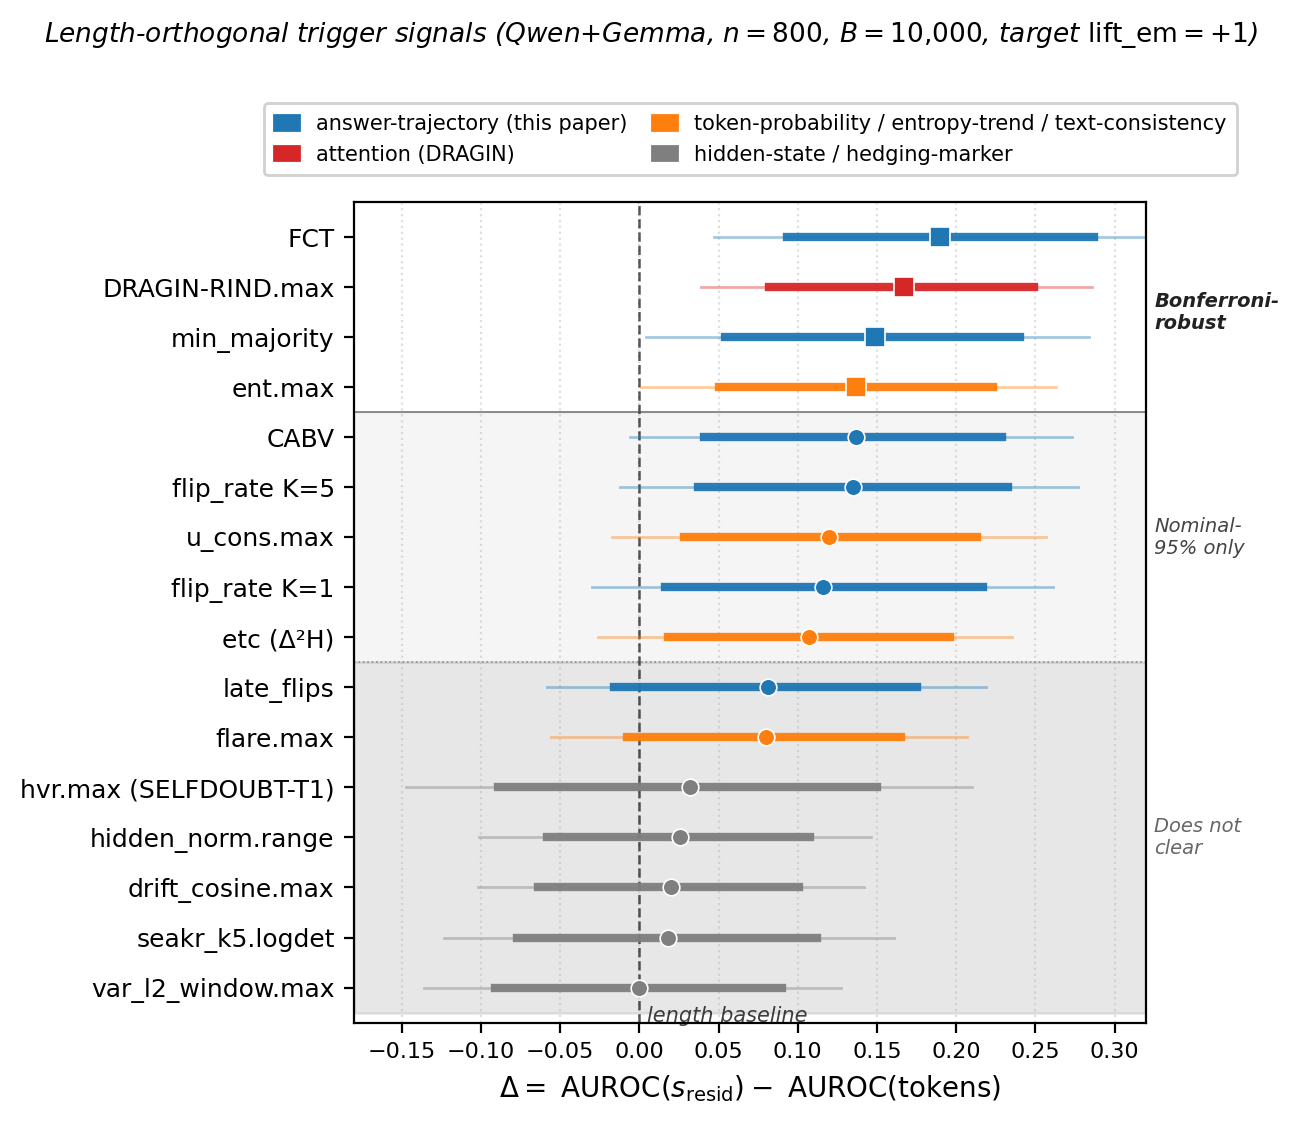
\includegraphics[width=\columnwidth]{figs/survivor_forest.png}
\caption{\textbf{Four trigger signals from three families carry length-orthogonal information beyond the length baseline; \textsc{FCT} (this paper) is strongest.} Forest plot of $\Delta = \mathrm{AUROC}(s_{\text{resid}}) - \mathrm{AUROC}(\texttt{tokens\_generated})$ on $\texttt{lift\_em}{=}+1$ ($n{=}800$ paired traces). Thick bars: 95\% paired-bootstrap CIs; thin extensions: Bonferroni-corrected 99.67\% CIs at $k{=}15$. Setup: \S\ref{sec:methods}. Tables: App.~\ref{sec:appendix-bonferroni}, \ref{sec:appendix-hero}.}
\label{fig:survivor-forest}
\end{figure}

\section{Introduction}
\label{sec:intro}

Dynamic retrieval-augmented generation (RAG) systems retrieve external evidence during decoding to ground generation in source material \citep{lewis_retrieval-augmented_2021, trivedi_interleaving_2023, shao_enhancing_2023}. At the core of every such system sits a \emph{retrieval trigger}: a scalar function of the partial generation that decides when to fire retrieval, evaluated by ranking traces by the trigger score and reporting raw AUROC against a binary correctness label. We restrict our audit to \emph{training-free} triggers. Prior work spans six signal families: attention-based DRAGIN \citep{su_dragin_2024}, token-probability FLARE \citep{jiang_active_2023}, entropy-trend ETC \citep{li_modeling_2026}, hidden-state SeaKR \citep{yao_seakr_2025} and INSIDE \citep{chen_inside_2024}, multi-sample text-consistency ($U_{\text{cons}}$ component of RSUS, \citealp{guo_when_2026}), and hedging-marker SELFDOUBT-T1 \citep{pandey_selfdoubt_2026}. A contemporaneous answer-trajectory family tracks step-level dynamics of the model's own predicted answer \citep{datta_large_2026, wang_chain--probe_2025, chen_i_2026}. 

Recent work has shown this evaluation convention is length-confounded on adjacent QA selective-prediction and uncertainty-quantification (UQ) tasks. \citet{santilli_revisiting_2025} prove that mutual length-bias on UQ scores and correctness functions systematically distorts AUROC. \citet{janiak_illusion_2025} show the empirical consequence: detection AUROC drops by up to 45.9\% when switching from ROUGE to an LLM-as-Judge label. \citet{zhang_verbosity_2024} attribute the underlying behavior to verbosity compensation on multi-hop QA, and \citet{ielanskyi_addressing_2025} document a related correctness-function failure across approximate metrics. The methodological response is \citet{vashurin_uncertainty-line_2025}'s \textsc{Uncertainty-Line}, which regresses each UQ score on output length and uses the residual as a length-invariant estimate. The dynamic-RAG trigger pool is the missing application.

We extend the length-residualization protocol of \citet{vashurin_uncertainty-line_2025} to the training-free dynamic-RAG trigger pool. Rather than score triggers against single-arm correctness, we re-decode each closed-book trace under gold context and ask whether retrieval flips a wrong answer to a right one, defining a paired-oracle target $\texttt{lift\_em}{=}+1$ conceptually motivated by \citet{mallen_when_2023}. This isolates the \emph{causal} retrieval-helpfulness signal from the length-correlated incorrectness signal that the published pool actually measures (\S\ref{sec:discussion-causal}). We also propose \textbf{FCT} (first-commitment time), a forward-looking variant of the answer-trajectory primitive \citep{datta_large_2026, wang_chain--probe_2025, chen_i_2026, zhang_when_2026}. FCT reads $K{=}5$ majority answers from non-thinking-mode chat models, where neither Datta's \texttt{</think>}-anchored forced completion nor \citeauthor{zhang_when_2026}'s finite-set continuation projection applies directly (App.~\ref{sec:appendix-fct-tstar}). 

\paragraph{Contributions.} (1) A length-residualized audit of the dynamic-RAG trigger pool, the first to our knowledge, scored against a paired-oracle target ($\texttt{lift\_em}{=}+1$). (2) \textbf{FCT} (first-commitment time), our forward-looking variant of the answer-trajectory primitive and the strongest length-residualized trigger in the audited pool. (3) A correctness-function robustness check against \citet{janiak_illusion_2025} and \citet{ielanskyi_addressing_2025}, under which the survivor matrix is preserved and FCT \emph{strengthens}.

\section{Related Work}
\label{sec:related}

The length-confound critique of standard UQ AUROC evaluation comes from QA UQ and hallucination detection \citep{santilli_revisiting_2025, janiak_illusion_2025, zhang_verbosity_2024, ielanskyi_addressing_2025, vashurin_uncertainty-line_2025, mao_confidence_2026}. The answer-trajectory family \citep{datta_large_2026, wang_chain--probe_2025, chen_i_2026} provides the parent primitives for FCT. Two related supervised methods sit outside our training-free scope: \citet{lu_streaming_2026} train hidden-state probes for streaming hallucination detection, and \citet{zhang_harnessing_2026} contrastively shape answer embeddings under latent perturbation at the trace boundary, where their ``answer agreement'' differs from our $K{=}5$ boundary-completion ``answer-trajectory''. Trained adaptive-retrieval policies likewise fall outside our audit \citep{asai_self-rag_2023, guo_dior_2025}. Our paired-oracle target operationalizes the question of when retrieval helps a parametric model \citep{mallen_when_2023}, replacing static entity-popularity proxies with per-trace closed-vs-oracle re-decode.
\section{Methods}
\label{sec:methods}

\subsection{Paired-Oracle \texttt{lift\_em} Protocol}
\label{sec:methods-protocol}

The published trigger pool scores against single-arm correctness, a target length predicts moderately well on multi-hop QA (\S\ref{sec:discussion-causal}). We instead define a paired target that flags traces where retrieval would convert a wrong answer to right, isolating the \emph{causal} retrieval-helpfulness signal from length-correlated incorrectness. Concretely, for each question $q$, we run two greedy decodes on the same chat model: a closed-book pass that produces trace $\tau_c^{(q)}$ and answer $a_c^{(q)}$, and an oracle pass conditioned on the gold supporting paragraphs that produces $a_o^{(q)}$ (decoding prompts and answer-extraction details: App.~\ref{sec:appendix-prompts}). We read all trigger signals from $\tau_c^{(q)}$; the oracle decode only supplies the label. The discrimination target is

\begin{equation}
\texttt{lift\_em}(q) = \mathbb{1}\!\left[\mathrm{EM}(a_o^{(q)}) > \mathrm{EM}(a_c^{(q)})\right]
\label{eq:lift-em}
\end{equation}

We evaluate on HotpotQA \citep{yang_hotpotqa_2018} and 2WikiMultiHopQA \citep{ho_constructing_2020}, holding the latter out as a cross-dataset cell, at $n{=}200$ paired traces per architecture-by-dataset cell. The two models are Qwen2.5-7B-Instruct (dense) and Gemma-4-26B-A4B-it (MoE-hybrid), chosen for cross-architecture coverage. The positive class is rare: 108 of 800 paired traces, base rate $13.5\%$.

\subsection{Length Residualization}
\label{sec:methods-residualization}

We adopt the residualization protocol of \citet{vashurin_uncertainty-line_2025}. For each trigger signal $s$ on a cohort of paired traces, we fit OLS of $s$ on $\log(\texttt{tokens}+1)$ and evaluate AUROC on the residual:
\begin{equation}
s_{\text{resid}} = s - \hat{\alpha} - \hat{\beta}\,\log(\texttt{tokens} + 1).
\label{eq:residualize}
\end{equation}
Intuitively, $s_{\text{resid}}$ keeps only the part of $s$ that length cannot linearly explain; its AUROC therefore measures whether the signal carries information beyond length. Our $\log(\texttt{tokens}+1)$ parameterization agrees within $\varepsilon \leq 0.029$ AUROC with the public reference implementation on our cohorts (App.~\ref{sec:appendix-uline}). Several signals in the audited pool (ETC, FLARE, SeaKR, SELFDOUBT-T1) are originally online or per-token, and we evaluate each as a trace-level summary statistic with granularity adapters in Appendix~\ref{sec:appendix-adapters}.

\subsection{FCT and the Answer-Trajectory Family}
\label{sec:methods-fct}

At each reasoning-step boundary (detected by tokenizer-level sentence-end token matchings), we sample $K{=}5$ boundary completions at temperature $\tau{=}0.6$, top-$p$~0.9, and extract a per-step answer from each via a regex over the model's \texttt{Answer:} prefix (sampler config and extractor regex: App.~\ref{sec:appendix-prompts}). From the resulting per-step $K{=}5$ majority sequence $\mathcal{M} = (m_1, \ldots, m_n)$ we compute four trace-level aggregations:
\begin{itemize}
\item \texttt{flip\_rate}: fraction of consecutive-step majority disagreements;
\item \texttt{late\_flips}: count of $K{=}5$ answer-\emph{set} disagreements in the last half of the trace;
\item \texttt{min\_majority}: $1 - \min_t (\max_{\text{count}}/K)$, the worst within-step disagreement;
\item \textbf{FCT}, a forward-looking first-commitment time
\begin{equation}
\begin{aligned}
\textsc{FCT} &= \frac{t_{\text{commit}}}{\max(1, n - 1)} \in [0, 1], \\
t_{\text{commit}} &= \min\{\, k : m_j = a_{\text{final}} \;\forall\, j > k \,\},
\end{aligned}
\label{eq:fct}
\end{equation}
\noindent with $k \in \{0, \dots, n{-}1\}$.
\end{itemize}
\noindent High FCT denotes late convergence: traces that have not settled on a final answer until close to the end of the decode are the traces where retrieval is most likely to help (worked example: App.~\ref{sec:appendix-prompts}). All four aggregations adapt the \texttt{AnswerSwitches} primitive of \citet{datta_large_2026} to non-thinking-mode chat models with $K{=}5$ majority-answer extracts. Neither Datta's \texttt{</think>}-anchored forced completion nor \citeauthor{zhang_when_2026}'s finite-set continuation projection applies directly in this regime (App.~\ref{sec:appendix-fct-tstar}).

\section{Results}
\label{sec:results}

\subsection{Cross-Architecture Survivor Matrix}
\label{sec:results-matrix}

Of the 16 audited signals, nine clear the length baseline at nominal 95\% paired-bootstrap, and only four survive Bonferroni correction at $k{=}15$ (Figure~\ref{fig:survivor-forest}): attention-based DRAGIN-RIND ($\Delta = +0.167$), token-probability \texttt{ent.max} ($+0.137$), answer-trajectory \texttt{min\_majority} ($+0.149$), and \textbf{FCT} ($+0.190$, the strongest length-residualized trigger in the pool). The four survivors span three of the seven declared families, which suggests the length-orthogonal signal is not a quirk of any one mechanism. Two families have no nominal-95\% survivor: hidden-state (SeaKR, INSIDE, plus three geometry variants) and hedging-marker (SELFDOUBT-T1) are absorbed by length (App.~\ref{sec:appendix-spearman}). The full table is in App.~\ref{sec:appendix-hero}.

\subsection{Length Is Anti-Predictive on the Held-Out 2Wiki Cells}
\label{sec:results-inverted}

The Bonferroni-robust four answer one question: which signals beat length? A sharper question is when length itself stops being informative. On the two held-out 2Wiki cells, raw answer length is at or below chance for predicting retrieval need: \texttt{tokens\_generated} reaches AUROC \textbf{0.457} on Qwen~$\times$~2Wiki and \textbf{0.518} on Gemma~$\times$~2Wiki. The verbosity-compensation pattern \citet{zhang_verbosity_2024} document on the same LongBench bundle does not transfer to \texttt{lift\_em}: longer multi-hop traces are no longer reliably retrieval-helpful. The four Bonferroni-robust survivors clear the length baseline by a wider margin on these cells than on HotpotQA, meaning the raw-AUROC protocol miscounts the length signal on exactly the cells where retrieval matters most.

\subsection{FCT Discriminates Strongest on the Held-Out MoE Cell}
\label{sec:results-fct-percell}

The cells where length fails are the cells where FCT succeeds. On Gemma~$\times$~2Wiki, the held-out cell where length is closest to chance (\texttt{tokens\_generated} 0.518), FCT reaches raw AUROC \textbf{0.784}, a $+0.266$ absolute gap over length (Table~\ref{tab:fct-percell}). The same pattern repeats on Qwen~$\times$~2Wiki: where the length proxy is below chance (0.457), FCT's margin ($+0.147$) is wider than on either HotpotQA cell. The answer-trajectory primitive carries the most independent information where the length proxy collapses.

\begin{table}[h]
\centering\small
\begin{tabular}{@{}lrrr@{}}
\toprule
\textbf{Cell} & $n$ & \textbf{helped} & \textbf{FCT AUROC} \\
\midrule
Qwen $\times$ HotpotQA  & 200 & 31 & 0.677 \\
Qwen $\times$ 2Wiki     & 200 & 34 & 0.604 \\
Gemma $\times$ HotpotQA & 200 & 19 & 0.642 \\
\textbf{Gemma $\times$ 2Wiki} & 200 & 24 & \textbf{0.784} \\
\bottomrule
\end{tabular}
\caption{Per-cell raw AUROC of FCT on $\texttt{lift\_em}{=}+1$.}
\label{tab:fct-percell}
\end{table}

\subsection{Survivor Set Is Robust to a Semantic-Equivalence Judge}
\label{sec:results-llmjudge}

The natural alternative explanation for the survivor matrix is that it reflects EM's string-matching artifact rather than a length-orthogonal signal. To rule this out we relabelled both arms of every paired trace via a GPT-4o-Mini judge (\citeauthor{janiak_illusion_2025}'s exact choice) and re-ran the audit, addressing the correctness-function critique of \citet{janiak_illusion_2025} and \citet{ielanskyi_addressing_2025}. EM and the judge agree at Cohen's $\kappa = 0.707$ (substantial agreement; \citealp{landis_measurement_1977}). Eight of the nine paired-significant survivors under EM remain significant under the judge, with a single swap (\texttt{etc} loses, \texttt{flare.max} gains) that leaves the Bonferroni-robust four intact. FCT itself \emph{strengthens} under the judge from $\Delta = +0.190$ to $\Delta = +0.222$, the opposite of what a string-level EM artifact would predict under semantic relabeling (App.~\ref{sec:appendix-llmjudge}).

\subsection{The $K{=}5$ Multi-Sample Variant Is Null}
\label{sec:results-ablation}

The paired-bootstrap CI on $\Delta_{K{=}5 - K{=}1}$ for \texttt{flip\_rate} straddles zero on both architectures (Qwen $-0.002$, $[-0.040, +0.031]$; Gemma $+0.033$, $[-0.025, +0.092]$; App.~\ref{sec:appendix-k-ablation}). The audit reports $K{=}5$ throughout because that was the capture protocol when the ablation returned null; for deployment $K{=}1$ delivers the same triggering performance at $5\times$ less compute per boundary. $K{=}1$ here is a single stochastic sample at the same ($\tau{=}0.6$, top-$p{=}0.9$); a deterministic-greedy $K{=}1$ ablation is left to future work.

\section{Discussion}
\label{sec:discussion}

\subsection{Why Length Predicts Retrieval-Helpfulness}
\label{sec:discussion-causal}

On the secondary $\texttt{closed\_em}{=}0$ target, \texttt{tokens\_generated} reaches raw AUROC $0.539$ on the headline pool, competitive with several internal signals. This pattern matches \citet{zhang_verbosity_2024}'s verbosity-compensation mechanism. A plausible causal chain is $\text{length} \rightarrow \text{verbosity compensation} \rightarrow \text{uncertainty} \rightarrow \text{incorrectness} \rightarrow \text{retrieval need}$, and length predicts $\texttt{closed\_em}{=}0$ moderately well because it proxies the upstream incorrectness step. The paired-oracle target $\texttt{lift\_em}{=}+1$ strips that step by conditioning on closed-book wrongness, which is why length collapses on the held-out 2Wiki cells (\S\ref{sec:results-inverted}).

\subsection{Why Answer-Trajectory Stability Predicts Retrieval Need}
\label{sec:discussion-fct}

The mechanism behind FCT reads naturally as \emph{premature commitment}, the interpretation \citet{datta_large_2026} give to their \texttt{AnswerSwitches} and $t^\star$ primitives. The model decides on an answer early and continues to verbalize reasoning that supports the commitment, with most subsequent steps as post-decision tail. \citeauthor{datta_large_2026} apply this observation to early stopping: if the model has decided, no further compute is needed. Retrieval triggering reads the same primitive in the opposite causal direction. The traces where the model has not decided, where the answer trajectory continues to flip through the reasoning, are exactly the traces where external evidence would resolve the uncertainty. The paired-oracle target $\texttt{lift\_em}{=}+1$ formalizes that question directly. The same primitive supports two complementary operations: detect stabilization to \emph{stop}, detect non-stabilization to \emph{retrieve}.

\section{Conclusion}
\label{sec:conclusion}

We presented the first length-residualized audit of the dynamic-RAG trigger pool, extending the protocol of \citet{vashurin_uncertainty-line_2025} to a paired-oracle target ($\texttt{lift\_em}{=}+1$). On two open-weight chat models over HotpotQA and 2WikiMultiHopQA, nine signals beat the length baseline at 95\% paired-bootstrap and four survived Bonferroni at $k{=}15$ across three families. The strongest length-residualized trigger is \textbf{FCT}, our forward-looking variant of the answer-trajectory primitive, exceeding length by $\Delta = +0.190$ AUROC and reaching raw $0.784$ on the held-out Gemma~$\times$~2Wiki cell. The survivor set is robust to a GPT-4o-Mini semantic-equivalence judge ($\kappa = 0.707$), with FCT itself strengthening under the judge. The same answer-trajectory primitive supports two complementary deployment operations: detect stabilization to \emph{stop}, detect non-stabilization to \emph{retrieve}.

\section*{Limitations}
\label{sec:limitations}

\paragraph{Signal-level audit, not end-to-end pipelines.} We audit trigger \emph{signals} as defined in their original papers, not full deployment pipelines (threshold tuning, retriever choice, prompt format). Our claims pertain to signal-level discriminative power on $\texttt{lift\_em}$.

\paragraph{Bonferroni knife-edge.} Two of the four Bonferroni-robust survivors (\texttt{ent.max}, \texttt{min\_majority}) carry $\sim$99.67\% lower bounds within $5{\times}10^{-3}$ of zero (App.~\ref{sec:appendix-bonferroni}). The four-survivor count is therefore fragile to small perturbations. The FCT and DRAGIN-RIND lower bounds are robust at $+0.047$ and $+0.039$.

\paragraph{Architecture and dataset coverage.} The headline pool covers two architectures and two multi-hop QA benchmarks. The cheapest extensions are a third open-weight chat model (e.g., Llama-3.1-8B-Instruct) and a third multi-hop benchmark (MuSiQue, \citealp{trivedi__2022}). The current FCT Bonferroni lower bound ($+0.047$) is the statistical floor additional cells would have to displace.

\paragraph{Dataset framing: held-out, not OOD.} We treat 2WikiMultiHopQA as a \emph{held-out} cell relative to HotpotQA, not as out-of-distribution in the strict sense: both are multi-hop QA over Wikipedia with comparable question complexity. The cell-dependent length behavior (\S\ref{sec:results-inverted}) is a dataset-specific finding on multi-hop QA rather than a claim about OOD generalization, and a stricter cross-distribution evaluation is future work.

\paragraph{Correctness function.} We use exact-match equality on both arms of the paired-oracle target. The paired design (\S\ref{sec:methods-protocol}) and the LLM-as-Judge robustness check (App.~\ref{sec:appendix-llmjudge}) partially insulate the headline against this choice. Containment-match and $F_1$ variants remain future work.

\paragraph{Non-thinking-mode chat models.} The audited models are non-thinking-mode chat variants. \citet{datta_large_2026} developed their answer-trajectory primitive on thinking-mode reasoning models with explicit \texttt{</think>} tokens. Our $K{=}5$ boundary-completion adaptation is not byte-faithful to that protocol.

\paragraph{Risks.} Our work concerns evaluation methodology for retrieval triggering on open-weight chat models and public multi-hop QA benchmarks. We release no new datasets or trained models, and direct risks are limited. One methodological risk is that the length-residualized protocol could be cited in isolation to defend deployed dynamic-RAG systems whose triggers track length more strongly than residualization alone would reveal. We therefore recommend reporting raw, length-residualized, and LLM-judge-validated AUROC together (\S\ref{sec:results-llmjudge}) rather than substituting one for another.

% Bibliography
\bibliography{custom}

\appendix

\section{Bonferroni-Corrected Survivor Set}
\label{sec:appendix-bonferroni}

Table~\ref{tab:bonferroni} reports the Bonferroni-corrected $\sim$99.67\% paired-bootstrap CI of $\Delta = \mathrm{AUROC}(s_{\text{resid}}) - \mathrm{AUROC}(\texttt{tokens\_generated})$ at $k{=}15$ ($\alpha = 0.05/15 = 0.0033$) on the headline pool. Bonferroni $k$ is the number of signals tested for the survivor-matrix claim. Four signals retain a strictly positive lower CI bound under correction: FCT, DRAGIN-RIND, \texttt{min\_majority}, and \texttt{ent.max}.\footnote{$k{=}15$ was the multiple-comparison count fixed at test time, when the audited pool included a CABV$\times$LAAS composite that we later dropped from presentation (\S\ref{sec:methods-fct}). The current table reports 16 audited signals plus the length baseline. The Bonferroni-corrected CI half-widths in the table ($\approx 0.12$--$0.14$ AUROC at $B{=}10{,}000$) dominate any plausible $k$-sensitivity at this signal pool size. We report the test as run.}

\begin{table}[h]
\centering
\resizebox{\columnwidth}{!}{%
\begin{tabular}{@{}lrll@{}}
\toprule
\textbf{Signal} & $\boldsymbol{\Delta}$ & \textbf{95\% CI} & \textbf{99.67\% CI (Bonf.)} \\
\midrule
\multicolumn{4}{l}{\textit{Bonferroni-robust:}} \\
\midrule
\textbf{FCT}              & $+0.190$ & $[+0.093, +0.287]$ & $[+0.047, +0.329]$ \\
\textbf{DRAGIN-RIND}      & $+0.167$ & $[+0.082, +0.249]$ & $[+0.039, +0.286]$ \\
\textbf{min\_majority}    & $+0.149$ & $[+0.054, +0.240]$ & $[+0.004, +0.284]$ \\
\textbf{ent.max}          & $+0.137$ & $[+0.050, +0.223]$ & $[+0.001, +0.263]$ \\
\midrule
\multicolumn{4}{l}{\textit{Nominal-95\% only:}} \\
\midrule
CABV                      & $+0.137$ & $[+0.041, +0.229]$ & $[-0.006, +0.273]$ \\
flip\_rate $K{=}5$        & $+0.135$ & $[+0.037, +0.233]$ & $[-0.012, +0.277]$ \\
u\_cons.max               & $+0.120$ & $[+0.028, +0.213]$ & $[-0.017, +0.257]$ \\
flip\_rate $K{=}1$        & $+0.116$ & $[+0.016, +0.217]$ & $[-0.030, +0.261]$ \\
etc ($\Delta^2 H$)        & $+0.107$ & $[+0.018, +0.196]$ & $[-0.026, +0.235]$ \\
\bottomrule
\end{tabular}%
}
\caption{Bonferroni-corrected survivor set on the headline pool (Qwen+Gemma, $n{=}800$ paired, $\texttt{lift\_em}{=}+1$, $B{=}10{,}000$). The \texttt{etc} ($\Delta^2 H$) signal is the Entropy-Trend Constraint trigger of \citet{li_modeling_2026}. CABV (continuous answer-belief velocity) is defined in App.~\ref{sec:appendix-cabv}.}
\label{tab:bonferroni}
\end{table}

\section{Full Headline Survivor Matrix}
\label{sec:appendix-hero}

Table~\ref{tab:hero-full} reports all 16 audited signals on the headline pool with length-residualized AUROC and $\Delta$ vs.\ \texttt{tokens\_generated}.

\begin{table*}[t]
\centering\small
\begin{tabular}{@{}llrcl@{}}
\toprule
\textbf{Signal} & \textbf{Family} & \textbf{Resid AUROC} & $\boldsymbol{\Delta}$ \textbf{vs.\ tokens} & \textbf{95\% CI} \\
\midrule
\texttt{tokens\_generated} & length            & 0.531 & --- & (baseline) \\
\midrule
\textbf{FCT}              & answer-trajectory & 0.691 & $+0.190$ & $[+0.093, +0.287]$ \\
\textbf{DRAGIN-RIND}      & attention         & 0.640 & $+0.167$ & $[+0.082, +0.249]$ \\
\textbf{min\_majority}    & answer-trajectory & 0.626 & $+0.149$ & $[+0.054, +0.240]$ \\
\textbf{ent.max}          & token-probability & 0.611 & $+0.137$ & $[+0.050, +0.223]$ \\
CABV                      & answer-trajectory & 0.641 & $+0.137$ & $[+0.041, +0.229]$ \\
flip\_rate $K{=}5$        & answer-trajectory & 0.640 & $+0.135$ & $[+0.037, +0.233]$ \\
u\_cons.max               & $K{=}3$ text      & 0.593 & $+0.120$ & $[+0.028, +0.213]$ \\
flip\_rate $K{=}1$        & answer-trajectory & 0.621 & $+0.116$ & $[+0.016, +0.217]$ \\
etc ($\Delta^2 H$)        & entropy-trend     & 0.580 & $+0.107$ & $[+0.018, +0.196]$ \\
\midrule
late\_flips               & answer-trajectory & 0.586 & $+0.081$ & $[-0.016, +0.175]$ \\
flare.max                 & token-probability & 0.553 & $+0.080$ & $[-0.008, +0.165]$ \\
hvr.max (SELFDOUBT-T1)\,\citep{pandey_selfdoubt_2026}    & hedging-marker    & 0.505 & $+0.032$ & $[-0.089, +0.150]$ \\
hidden\_norm.range        & hidden (geom.)    & 0.499 & $+0.026$ & $[-0.058, +0.108]$ \\
drift\_cosine.max         & hidden (geom.)    & 0.493 & $+0.020$ & $[-0.064, +0.101]$ \\
seakr\_k5.logdet          & $K{=}5$ hidden    & 0.491 & $+0.018$ & $[-0.077, +0.112]$ \\
var\_l2\_window.max       & hidden (geom.)    & 0.473 & $+0.000$ & $[-0.091, +0.090]$ \\
\bottomrule
\end{tabular}
\caption{Full cross-architecture survivor matrix on the headline pool (Qwen2.5-7B + Gemma-4-26B-A4B-it $\times$ \{HotpotQA, 2WikiMHQA\}, $n{=}800$ paired traces). All AUROCs are length-residualized (\S\ref{sec:methods-residualization}). 95\% CIs are paired-bootstrap ($B{=}10{,}000$) of $\Delta = \mathrm{AUROC}(s_{\text{resid}}) - \mathrm{AUROC}(\texttt{tokens\_generated})$. \textbf{Bold}: Bonferroni-robust at $k{=}15$ (lower bound of the 99.67\% CI strictly positive; see Table~\ref{tab:bonferroni}).}
\label{tab:hero-full}
\end{table*}

\section{Correctness-Function Robustness: LLM-as-Judge}
\label{sec:appendix-llmjudge}

\paragraph{Protocol.} For each of the $n{=}800$ paired traces in the headline pool, we re-labelled both arms via an OpenAI \texttt{gpt-4o-mini} semantic-equivalence judge under a strict three-sentence system prompt: ``You are a strict semantic-equivalence judge for multi-hop QA. Your task is to decide whether a model-predicted answer is semantically equivalent to a gold answer. Reply with exactly one word: YES or NO. No explanation.'' The judge target is
\begin{equation}
\texttt{lift\_em}_{\textsc{judge}}(q) = \mathbb{1}\!\bigl[\mathrm{judge}(a_o^{(q)}){=}\textsc{YES} \;\wedge\; \mathrm{judge}(a_c^{(q)}){=}\textsc{NO}\bigr].
\label{eq:lift-em-judge}
\end{equation}
We re-ran the full headline survivor matrix with paired bootstrap $B{=}10{,}000$.

\paragraph{Inter-label agreement.} EM identifies 108 helped traces and the judge identifies 113; the intersection is 87. The two labels jointly produce a multi-class Cohen's $\kappa = 0.707$ on the 3-class $\texttt{lift\_em} \in \{+1, 0, -1\}$ label set, in the substantial-agreement band of \citet{landis_measurement_1977}.

\paragraph{Survivor matrix transfer.} Table~\ref{tab:llmjudge} reports the headline survivor matrix under both correctness functions side-by-side. Eight of the nine paired-significant survivors under EM remain significant under the judge, with a single swap: \texttt{etc} loses significance and \texttt{flare.max} gains it. FCT strengthens under the judge from $\Delta = +0.190$ [+0.093, +0.287] to $\Delta = +0.222$ [+0.132, +0.312] ($+17\%$ in point estimate, $+42\%$ in 95\% CI lower-bound margin), the opposite of what a string-level EM artifact would predict. All four Bonferroni-robust survivors retain nominal-95\% significance under the judge.

\begin{table}[h]
\centering\small
\begin{tabular}{@{}lll@{}}
\toprule
\textbf{Signal} & $\boldsymbol{\Delta}_{\textsc{em}}$ & $\boldsymbol{\Delta}_{\textsc{judge}}$ \\
\midrule
\textbf{FCT}              & $+0.190$         & $\mathbf{+0.222}$ \\
\textbf{DRAGIN-RIND}      & $+0.167$         & $+0.157$ \\
\textbf{min\_majority}    & $+0.149$         & $+0.155$ \\
\textbf{ent.max}          & $+0.137$         & $+0.125$ \\
CABV                      & $+0.137$         & $+0.177$ \\
flip\_rate $K{=}5$        & $+0.135$         & $+0.178$ \\
u\_cons.max               & $+0.120$         & $+0.157$ \\
flip\_rate $K{=}1$        & $+0.116$         & $+0.171$ \\
etc ($\Delta^2 H$)        & $+0.107$         & $+0.088^{\ast}$ \\
flare.max                 & $+0.080^{\ast}$  & $+0.115$ \\
\bottomrule
\end{tabular}
\caption{Side-by-side $\Delta$ under EM and LLM-as-Judge on the headline pool ($n{=}800$, $B{=}10{,}000$). $^{\ast}$95\% CI straddles zero. FCT \emph{strengthens} under the judge. Eight of nine paired-significant EM survivors are preserved, and all four Bonferroni-robust survivors retain nominal-95\% significance.}
\label{tab:llmjudge}
\end{table}

\paragraph{Caveat.} \citet{zheng_judging_2023} document that GPT-4-tier judges exhibit a verbosity bias, preferring longer responses; our cross-judge check demonstrates \emph{pattern stability} rather than full verbosity-independence. The load-bearing length-orthogonality argument rests on the \textsc{Uncertainty-Line} residualization (\S\ref{sec:methods-residualization}) and the paired-oracle design (\S\ref{sec:methods-protocol}); the judge check confirms the survivor matrix is not an artifact of any single correctness function.


\section{Decoding Prompts, Answer Extraction, and a Worked Example}
\label{sec:appendix-prompts}

\paragraph{Closed-book and oracle decoding.} Both arms of the paired-oracle target (\S\ref{sec:methods-protocol}) use a single chat-template message pair with a system role and a user role; the oracle arm differs only by paragraph filtering (gold supporting paragraphs only, distractors removed). Decoding is greedy ($\arg\max$ over post-repetition-penalty logits with \texttt{repetition\_penalty}~$=1.0$ on both architectures), \texttt{max\_new\_tokens}~$=1024$, with early stop on EOS or the first \texttt{Answer:\,$\langle$...$\rangle$\textbackslash n} line (checked every 16 generated tokens to amortize the decode cost). The shared system instruction is

\begin{quote}\small\itshape
You are a careful reasoner. Read the provided paragraphs, think step by step, and answer the question concisely. End your response with a single line of the form \mbox{`Answer: $\langle$your answer$\rangle$'} where $\langle$your answer$\rangle$ is as short as possible (typically 1--5 words).
\end{quote}

\noindent and the user payload is rendered as

\begin{quote}\small\ttfamily
Paragraphs:\\[1pt]
\mbox{[Paragraph 1: $\langle$Title 1$\rangle$]}\\
$\langle$Body 1$\rangle$\\[1pt]
\mbox{[Paragraph 2: $\langle$Title 2$\rangle$]}\\
$\langle$Body 2$\rangle$\\[1pt]
\dots\\[1pt]
Question: $\langle$Q$\rangle$\\[1pt]
Reason step by step, then end with \mbox{`Answer: ...'}.
\end{quote}

\noindent Both messages are rendered through each model's native chat template via Hugging Face \texttt{apply\_chat\_template} with default kwargs (no thinking-mode toggle on either model; Qwen2.5 has none, Gemma-4-26B-A4B-it leaves the thought channel empty under defaults). On HotpotQA the closed-book arm sees all 10 distractor paragraphs; the oracle arm sees only paragraphs whose title appears in the gold \texttt{supporting\_facts} (typically 2). Per-step boundary detection fires on tokenizer-level sentence-end tokens (period, newline, etc.) with a 32-token cap.

\paragraph{$K{=}5$ boundary completions.} At each detected boundary, the model state is forked from the cached \texttt{past\_key\_values} and 5 continuations are sampled at $\tau{=}0.6$, top-$p{=}0.9$, \texttt{max\_new\_tokens}~$=40$, multinomial over the nucleus, with the cache truncated back to the boundary on exit. Random seed $20260511$ is offset per step. The same $K{=}5$ samples feed both the answer-trajectory family (\S\ref{sec:methods-fct}) and the SeaKR-K=5 hidden proxy (App.~\ref{sec:appendix-adapters}).

\paragraph{Trace-level answer extraction.} The final-answer extractor scans for the \emph{last} occurrence of one of \{\texttt{final answer:}, \texttt{final\_answer:}, \texttt{answer:}, \texttt{\#\# answer}, \texttt{**answer**}, \texttt{**final answer**}\} (case-insensitive) whose payload does not begin with a placeholder echo (\texttt{<} or \texttt{[}), takes the first non-empty line, truncates at the first sentence-end punctuation followed by whitespace, splits at the first lower\texttt{->}upper seam past character 1 (defensive against decode-loop concatenation artefacts), and hard-caps at 100 characters. EM uses HotpotQA-standard SQuAD normalization: lowercase, strip articles ($\{a, an, the\}$), drop punctuation, collapse whitespace.

\paragraph{Per-step answer extraction (FCT input).} The per-step answer regex is intentionally tighter and faster, since it runs $5n$ times per trace:
\begin{quote}\small\ttfamily
\textbackslash bAnswer\textbackslash s*:\textbackslash s*(.+?)(?:[\textbackslash n.]|\$)
\end{quote}
\noindent (\texttt{re.IGNORECASE}). Per-step normalization keeps only \texttt{[a-z0-9 ]}, lowercases, and truncates at 30 characters. Per-step majority is \texttt{Counter(answers).most\_common(1)[0][0]}; FCT (Eq.~\ref{eq:fct}) is then the smallest index $t_{\text{commit}}$ such that every populated step at or after $t_{\text{commit}}$ has majority equal to the trace-level final answer, normalized by $\max(1, n_{\text{populated}}{-}1)$.

\paragraph{Worked example.} Qwen2.5-7B-Instruct $\times$ HotpotQA, question \texttt{5abd01205542992ac4f3819b} (a real \texttt{lift\_em}${=}{+}1$ trace from the headline pool):
\begin{quote}\small
\textbf{Q:} ``Mummulgum is a stop on the Bruxner Highway before reaching the town on the banks of which river?''\\
\textbf{Gold:} \emph{Richmond}\\
\textbf{Closed-book final answer:} \emph{Casino} (EM${=}0$)\\
\textbf{Oracle final answer:} \emph{Richmond} (EM${=}1$)\\
$\Rightarrow$ \texttt{lift\_em}${=}{+}1$.
\end{quote}
The closed-book trace has $n{=}3$ step boundaries. Per-step $K{=}5$ majority answers extracted from the boundary completions:
\begin{center}\small
\begin{tabular}{@{}rll@{}}
\toprule
\textbf{step} & \textbf{$K{=}5$ extracted answers} & \textbf{majority} \\
\midrule
1 & \{\texttt{casino}\} (1/5 emit \texttt{Answer:})       & \texttt{casino} \\
2 & \{\texttt{casino}$\times$4, \texttt{richmond river}\} & \texttt{casino} \\
3 & \{\texttt{casino}$\times$5\}                          & \texttt{casino} \\
\bottomrule
\end{tabular}
\end{center}
\noindent All three step-majorities equal the trace-level final answer (\texttt{casino}), so $t_{\text{commit}}{=}0$ and \textbf{FCT} ${=}\,0/(3{-}1){=}0.000$. This trace is a per-trace \emph{false negative} for FCT: the model committed to a wrong answer early, a mode FCT cannot distinguish from confident-correct early commitment. Aggregate FCT raw AUROC on \texttt{lift\_em}${=}{+}1$ is $0.784$ on Gemma~$\times$~2Wiki (Table~\ref{tab:fct-percell}); the Bonferroni 99.67\% lower bound is $+0.047$ (Table~\ref{tab:bonferroni}). FCT is the strongest length-residualized discriminator in the audited pool, not a per-trace oracle. The full trace JSON (closed and oracle arms, all 5 boundary samples per step, per-token logprobs, per-step entropies, hidden-state captures, gate decisions) will be released with the code (App.~\ref{sec:appendix-repro}).

\section{Uncertainty-Line Reference Replication}
\label{sec:appendix-uline}

To pre-empt the reimplementation critique, we ran our protocol (Eq.~\ref{eq:residualize}) and the \citet{vashurin_uncertainty-line_2025} reference implementation side-by-side on the same trace cohort, decomposing the comparison into two $\varepsilon$ components. $\varepsilon_{\text{protocol}}$ isolates the math difference (our $\log(\texttt{tokens}+1)$ single-cohort OLS against the reference MinMax-scaled linear regression on the same cohort); $\varepsilon_{\text{sampling}}$ isolates train/test-split sampling noise at $n{=}200$ (Table~\ref{tab:uline-repl}).

\begin{table}[h]
\centering\small
\begin{tabular}{@{}lrrrr@{}}
\toprule
\textbf{Arch} & $\varepsilon^{\text{prot}}_{\max}$ & $\varepsilon^{\text{prot}}_{\text{mean}}$ & $\varepsilon^{\text{prot}}_{\text{med}}$ & $\varepsilon^{\text{samp}}_{\max}$ \\
\midrule
Qwen2.5  & 0.029 & 0.012 & 0.012 & 0.111 \\
Gemma    & 0.027 & 0.0095 & 0.0047 & 0.106 \\
\bottomrule
\end{tabular}
\caption{$\varepsilon_{\text{protocol}} = |\text{ours}_{\text{resid}} - \text{LINE}_{\text{full}}|$; $\varepsilon_{\text{sampling}} = |\text{LINE}_{\text{full}} - \text{LINE}_{\text{split}}|$ (latter averaged over 3 seeds). Both architectures show $\varepsilon_{\text{protocol}} \leq 0.029$, well below the conventional threshold of $0.05$. Train/test sampling noise ($\varepsilon_{\text{sampling}}$) dominates the protocol gap by a factor of $3$--$4\times$, indicating that the $\log(\texttt{tokens}+1)$ vs.\ raw-MinMax math difference is small relative to evaluation-set variance at $n{=}200$.}
\label{tab:uline-repl}
\end{table}

\section{FCT vs.\ Concurrent Commitment-Time Primitives: Operational Differences}
\label{sec:appendix-fct-tstar}

FCT (\S\ref{sec:methods-fct}) is motivated by the final-switch index $t^\star = \max\{i : A_i \neq A_{i+1}\}$ of \citet{datta_large_2026}, with a concurrent forward-looking commitment-time primitive proposed by \citet{zhang_when_2026} on the model's finite-answer continuation distribution. The three are operationally distinct on five axes (Table~\ref{tab:fct-vs-tstar}).

\begin{table}[h]
\centering
\resizebox{\columnwidth}{!}{%
\begin{tabular}{@{}llll@{}}
\toprule
\textbf{Axis} & \textbf{Datta} $\boldsymbol{t^\star}$ & \textbf{Zhang} $\boldsymbol{\tau_{\text{commit}}}$ & \textbf{FCT (ours)} \\
\midrule
Temporal direction & Backward (last switch) & Forward (first stable) & Forward (first stable) \\
Signal class       & Per-step answer & Continuation log-odds & $K{=}5$ majority answer \\
Sampling regime    & $K{=}1$ forced-completion & Single deterministic state & $K{=}5$ stochastic \\
Application target & Early stopping & Pre-verbalization commitment & Retrieval triggering \\
Trace model class  & Thinking (\texttt{</think>}) & Delayed-verdict templates & Non-thinking chat \\
\bottomrule
\end{tabular}%
}
\caption{Operational differences across three concurrent commitment-time primitives. \citet{datta_large_2026}'s $t^\star$ is backward-looking on per-step intermediate answers, applied to early stopping. \citet{zhang_when_2026}'s $\tau_{\text{commit}}$ is forward-looking on the model's finite-answer continuation distribution (log-odds in binary tasks), applied to pre-verbalization commitment analysis. FCT (ours) is forward-looking on $K{=}5$-majority answer extracts, applied to retrieval triggering. For monotonically converging trajectories, $t_{\text{commit}} \approx t^\star + 1$; under $K{=}5$ majority sampling on non-thinking-mode chat models this equivalence does not hold in general.}
\label{tab:fct-vs-tstar}
\end{table}

\section{CABV: Continuous Answer-Belief Velocity}
\label{sec:appendix-cabv}

CABV is a continuous between-step generalization of \texttt{flip\_rate}: at each populated step we build a Laplace-smoothed empirical distribution over the trace's $K{=}5$ answers and average the Jensen--Shannon divergence between consecutive steps. CABV reduces to \texttt{flip\_rate} when each step concentrates on a single answer, and is closest in spirit to the inference-time instability signal of \citet{chen_i_2026}, defined on JSD between token distributions rather than $K{=}5$ answer distributions.

\section{Length-vs-Signal Spearman $\rho$ per Cell}
\label{sec:appendix-spearman}

Table~\ref{tab:spearman} reports Spearman $\rho$ between \texttt{tokens\_generated} and each signal per (arch $\times$ dataset) cell on closed-book traces, the length-confound diagnostic of \citet{santilli_revisiting_2025} (their Table~2). $|\rho| \geq 0.5$ indicates a strong length confound on the signal.

\begin{table}[h]
\centering
\resizebox{\columnwidth}{!}{%
\begin{tabular}{@{}lrrrr@{}}
\toprule
\textbf{Signal} & \textbf{Q$\times$Hot} & \textbf{Q$\times$Wiki} & \textbf{G$\times$Hot} & \textbf{G$\times$Wiki} \\
\midrule
DRAGIN-RIND          & $+0.40$ & $+0.35$ & $+0.38$ & $+0.38$ \\
ent.max              & $+0.31$ & $+0.26$ & $+0.42$ & $+0.32$ \\
etc ($\Delta^2 H$)   & $+0.32$ & $+0.36$ & $+0.46$ & $+0.40$ \\
flare.max            & $+0.39$ & $+0.35$ & $+0.45$ & $+0.32$ \\
u\_cons.max          & $+0.40$ & $+0.31$ & $+0.37$ & $+0.39$ \\
seakr\_k5            & $+0.37$ & $+0.44$ & $+0.46$ & $+0.43$ \\
drift\_cosine.max    & $+0.20$ & $+0.18$ & $-0.07$ & $-0.01$ \\
var\_l2\_window.max  & $+0.19$ & $+0.23$ & $+0.22$ & $-0.00$ \\
hidden\_norm.range   & $+0.24$ & $+0.29$ & $+0.36$ & $+0.16$ \\
hvr.max              & n/a$^{\ast}$ & $+0.06$ & $+0.30$ & $\mathbf{+0.51}$ \\
\midrule
flip\_rate $K{=}5$   & $+0.22$ & $+0.12$ & $+0.21$ & $+0.35$ \\
flip\_rate $K{=}1$   & $+0.17$ & $+0.15$ & $+0.27$ & $+0.21$ \\
late\_flips          & $+0.29$ & $+0.37$ & $+0.25$ & $+0.30$ \\
min\_majority        & $+0.18$ & $+0.12$ & $+0.14$ & $+0.09$ \\
CABV                 & $+0.22$ & $+0.17$ & $+0.22$ & $+0.36$ \\
FCT                  & $+0.20$ & $+0.14$ & $+0.15$ & $+0.30$ \\
\bottomrule
\end{tabular}%
}
\caption{Spearman $\rho(\texttt{tokens\_generated}, \text{signal})$ per cell on closed-book traces. Bold: $|\rho| \geq 0.5$. The peer-pool signals (DRAGIN, ent.max, etc, flare.max, u\_cons.max, seakr\_k5) carry $\rho \in [+0.26, +0.46]$, \texttt{hvr.max} reaches $+0.51$ on Gemma$\times$2Wiki, and the auxiliary hidden-state geometry diagnostics span $\rho \in [-0.07, +0.36]$. The answer-trajectory aggregations (bottom block) average $\approx 0.15$ lower in $|\rho|$ than the peer-pool block, the per-cell quantitative version of the family-level finding from \S\ref{sec:results-matrix}. $^{\ast}$Qwen$\times$Hot \texttt{hvr.max} is constant, so Spearman is undefined.}
\label{tab:spearman}
\end{table}

\section{$K{=}5$ vs.\ $K{=}1$ Ablation}
\label{sec:appendix-k-ablation}

Table~\ref{tab:k-ablation} reports the paired-bootstrap $\Delta_{K{=}5 - K{=}1}$ for \texttt{flip\_rate} on $\texttt{lift\_em}{=}+1$, pooled per architecture. Both CIs straddle zero (\S\ref{sec:results-ablation}).

\begin{table}[h]
\centering\small
\begin{tabular}{@{}lrrcc@{}}
\toprule
\textbf{Arch} & $n$ & \textbf{helped} & $\Delta_{K{=}5 - K{=}1}$ & \textbf{95\% CI} \\
\midrule
Qwen  & 305 & 47 & $-0.002$ & $[-0.040, +0.031]$ \\
Gemma & 394 & 42 & $+0.033$ & $[-0.025, +0.092]$ \\
\bottomrule
\end{tabular}
\caption{$K{=}5$ vs.\ $K{=}1$ \texttt{flip\_rate} ablation on $\texttt{lift\_em}{=}+1$, pooled per architecture.}
\label{tab:k-ablation}
\end{table}

\section{Adapter Notes}
\label{sec:appendix-adapters}

We audit signal-level discriminative power on \texttt{lift\_em} (\S\ref{sec:limitations}). Several primitives in the published trigger pool are originally framed as online per-token triggers or per-trace scores, and we evaluate their underlying statistic at the trace level on the closed-book trace $\tau_c^{(q)}$ decoded with the prompt of App.~\ref{sec:appendix-prompts}. The per-signal notes below state the original primitive, our trace-level adaptation, and any sign or granularity drift.

\paragraph{ETC \citep{li_modeling_2026}.} The original ETC operates on a token-level entropy stream; we evaluate $\Delta^2 H$ on the per-step mean entropy series captured at boundary-detection events (\S\ref{sec:methods-fct}). We score $\max |\Delta^2 H|$ rather than the signed second-difference, so the adapter is magnitude-faithful but not sign-faithful.

\paragraph{FLARE \citep{jiang_active_2023}.} The original FLARE is an online per-token retrieval trigger ($\max_t p_t < \tau$); we audit the underlying primitive (low-confidence detection) as a trace-level summary $\max$ over steps of $1 - \min p_t$. The trigger \emph{policy} is not audited; the trigger \emph{statistic} is.

\paragraph{SeaKR \citep{yao_seakr_2025}.} We use $K{=}5$ EOS hidden states for compute efficiency, smaller than the paper's reported best-$k$ interval $K \in [10, 25]$. The regularized Gram determinant we compute is the same primitive as the paper's self-aware uncertainty score. INSIDE \citep{chen_inside_2024} is the closest peer, using the EigenScore on the centered sample covariance; the $K$ nonzero eigenvalues of our uncentered Gram and INSIDE's centered covariance are rank-equivalent up to centering.

\paragraph{SELFDOUBT-T1 \citep{pandey_selfdoubt_2026}.} HVR $= h/(v+1)$ is computed per step from a fixed seed marker dictionary (\citeauthor{pandey_selfdoubt_2026} use a per-model Stage-2 expansion from the same seeds); we aggregate as $\max$ over steps and report AUROC of the continuous score. The original paper's Tier-1 ``HVR=0'' high-precision \emph{gate} is the binary degenerate ranking induced by threshold $0$ on this same statistic; we do not separately report gate precision/coverage. \citeauthor{pandey_selfdoubt_2026}'s evaluation is on multi-choice reasoning benchmarks (BBH, GPQA-Diamond, MMLU-Pro) over long thinking-mode traces, and they explicitly flag free-form generation as untested; our regime is short non-thinking-mode chat traces on multi-hop short-answer QA, so the audited result here measures HVR's transfer to a regime its authors flagged as untested.

\paragraph{Concurrent commitment-time primitives.} Operational differences between \citet{datta_large_2026}'s $t^\star$, \citet{zhang_when_2026}'s $\tau_{\text{commit}}$, and our FCT are tabulated in Appendix~\ref{sec:appendix-fct-tstar}.

\section{Reproducibility}
\label{sec:appendix-repro}

All decoding traces, paired closed-vs-oracle JSONLs, slice manifests with SHA-256 checksums, decoding command lines, and the LLM-as-Judge call cache will be released alongside the analysis scripts that produce every table and figure in this paper, including the worked example trace of App.~\ref{sec:appendix-prompts}. Compute: single NVIDIA A800 80\,GB, wall-clock $\sim$15\,h end-to-end.

\end{document}

